\section{Conclusión}

Cuestionario de conclusiones:

1. El control de “nivel de disparo” (trigger level) que todo osciloscopio posee en el panel frontal dentro de la sección de controles de la base de tiempos sirve para:\
\begin{enumerate}
	\item[A.] Ajustar el tiempo total del barrido.
	\item[B.] Ajustar el punto de inicio del barrido.
	\item[C.] Ajustar el punto de finalización del barrido.
	\item[D.] Ajustar la polaridad del punto de inicio o fin del barrido.
	\item[E.] Ajustar el tiempo de demora entre un barrido y el siguiente.
\end{enumerate}

\vspace{1em}

2. En el panel de controles de un osciloscopio típico, y dispuesto en la zona de controles de la base de tiempos, suele ubicarse el selector de “Fuente de disparo” cuya función es:\
\begin{enumerate}
\item[A.] Permite seleccionar entre disparo: LF (low frec.) o F (Higth frec.).
\item[B.] Permite seleccionar entre disparo: Automático -- Normal -- Único.
\item[C.] Permite seleccionar entre disparo: Interno -- Externo -- Línea.
\item[D.] Permite seleccionar entre disparo: CC -- CA.
\item[E.] Permite seleccionar entre disparo: Pendiente positiva -- Pendiente negativa.
\end{enumerate}

\vspace{1em}

3.	En un osciloscopio de doble trazo La presentación dual se logra mediante el empleo de una llave electrónica que actúa sobre los circuitos del eje vertical; esta llave puede trabajar en modo "Barrido alternado" (Alt.) o "Barrido troceado" (Troc.). Relacione cada uno de los modos, con las características que se listan:
\begin{enumerate}
\item[A.] Se emplea cuando la velocidad de barrido es elevada.
\item[B.] Se emplea cuando la velocidad de barrido es baja.
\item[C.] Dentro de cada ciclo de barrido se va alternado cada uno de los canales.
\item[D.] En un barrido se muestra un canal, y en el siguiente el otro
\end{enumerate}
\vspace{1em}
4.	En todos los osciloscopios de usos generales el disparo del barrido del eje X puede seleccionarse, al menos, entre “Modo automático” y “Modo normal”. En el modo normal, la base de tiempos se dispara cuando:
\begin{enumerate}
\item[A.] Hay señal presente en alguna de las entradas del eje Y.
\item[B.] El nivel de disparo está contenido entre el máximo y el mínimo de la señal de entrada.
\item[C.] Aunque no haya señal presente, se dispara mediante un pulso generado internamente.
\item[D.] El disparo se efectúa una vez, luego de lo cual se debe resetear la base de tiempos.
\end{enumerate}
\vspace{1em}
5.	En el panel de controles de todo osciloscopio, suele haber un punto de prueba (TP) donde hay disponible una señal, generada internamente, de 1KHz, con forma de onda cuadrada que según lo indicado habitualmente en los manuales se emplea para “calibra la punta de pruebas”. Dicho procedimiento se realiza:
\begin{enumerate}
\item[A.] Con la punta en posición X10 y es para calibrar la base de tiempos.
\item[B.] Con la punta en posición X10 y es para compensar la respuesta en frecuencia.
\item[C.] Con la punta en la posición X1 y es para compensar la respuesta en frecuencia.
\item[D.] Con la punta en la posición X1 y es para calibrar el nivel de disparo.
\end{enumerate}

\vspace{1em}

6.	La calibración de la punta, se hace observando la forma de onda cuadrada, y normalmente debe retocarse un ajuste que suele encontrarse:
\begin{enumerate}
\item[A.] En el panel del instrumento y se accede mediante un destornillador de plástico.
\item[B.] En la propia punta de pruebas, y se accede mediante un destornillador de plástico.
\item[C.] En la propia punta de pruebas, y para ello suele haber una llave de tres posiciones.
\item[D.] Debe retirarse la cubierta del osciloscopio ya que el ajuste suele estar en su interior.
\end{enumerate}
\vspace{1em}
7.	Por lo general todos los osciloscopios de doble trazo disponen, en el selector de “Modo Vertical”, de una posición denominada “ADD” (Suma). Este modo suele utilizarse juntamente con la opción “INV” (inversión) de uno de los canales Y. Cuando un osciloscopio se emplea de esta forma:
\begin{enumerate}
\item[A.] Es posible determinar la diferencia de fase entre dos señales de la misma frecuencia.
\item[B.] Funciona como un instrumento de canal único y entrada diferencial.
\item[C.] Permite visualizar una señal restando la componente de CC.
\item[D.] No es un modo que tenga utilidad. Debe ser evitado.
\end{enumerate}

\vspace{1em}

8.	La siguiente imagen representa un oscilograma obtenido con un osciloscopio, cuyos controles se encuentra en las siguientes posiciones: 
A.	Eje Y= 2V/div;
B.	Base de T = 1ms/div. 
C.	La sonda de pruebas se encuentra en la posición X 10, 
D.	La forma de onda observada no tiene componente de CC.
 
\begin{figure}[H]
    \centering
	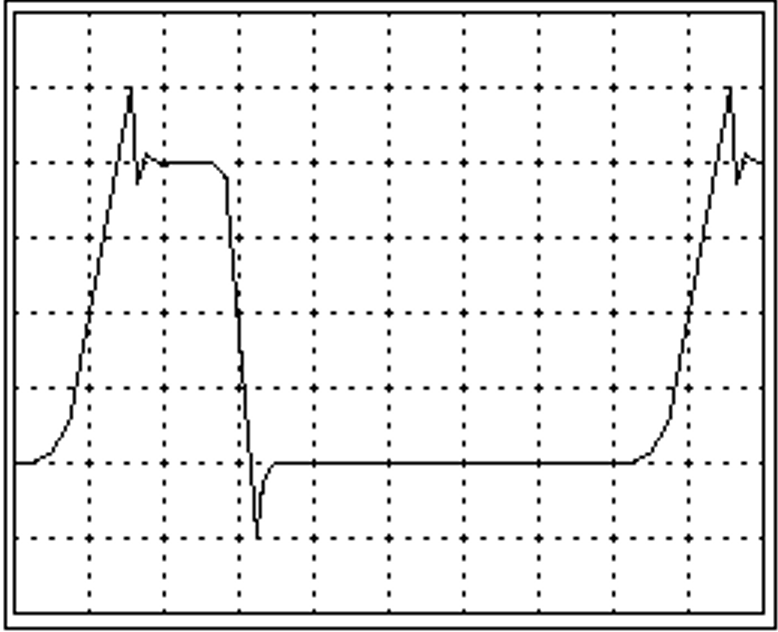
\includegraphics[width=0.4\textwidth]{images/conclusiones.png}
	\caption{Señal en x10 con acoplamiento en CA}
	\label{fig:calibracion}
\end{figure} 

E.	Se pide determinar:
\begin{enumerate}
\item[1.] El ciclo de trabajo de la forma de onda observada.
\item[2.] El valor eficaz de la tensión.
\end{enumerate}
